%\chapter*{Неделя 7}
\protect\thispagestyle{fancy}
\section{}
Используя теорему о свёртке во временной области для ДВПФ, определите линейную дискретную свёртку последовательностей:

\begin{align*}
	h[k] = \dfrac{\sin(2 \pi \nu_c k)}{\pi k},\quad \nu_c = 0.2;\quad x[k] = \cos(2\pi \nu_1 k) + \cos(2 \pi \nu_2 k), \quad \nu_1 = 0.1,\; \nu_2 = 0.3.
\end{align*}

Интерпретируйте результат как прохождение сигнала $x[k]$ через фильтр с импульсной характеристикой $h[k]$. Является ли такой фильтр $h[k]$ физически реализуемым?

\begin{equation*}
	h[k] \xlongleftrightarrow{DTFT} \Capit{H}(\nu) = \Theta\left(|\nu| \leq \nu_c\right) = 
	\begin{cases}
		1,& \text{если } m-\nu_c \leq \nu \leq m+\nu_c,\; m\in\mathbb{Z},\\
		0,& \text{иначе.}
	\end{cases}
\end{equation*}

\begin{equation*}
	x[k] \xlongleftrightarrow{DTFT} \Capit{X}(\nu) = \dfrac{1}{2}\sum\limits_{m = \infty}^{+\infty}
	\left[\delta(\nu - \nu_1 + m) + \delta(\nu + \nu_1 + m) + \delta(\nu - \nu_2 + m) + \delta(\nu + \nu_2 + m)\right].
\end{equation*}

\begin{align*}
	\Capit{Y}(\nu) &= \Capit{X}(\nu) \cdot \Capit{H}(\nu) = \dfrac{1}{2}\sum\limits_{m = -\infty}^{+\infty}
	\Theta_m\left(|\nu| \leq \nu_c\right) \left[\delta(\nu - \nu_1 + m) + \delta(\nu + \nu_1 + m) + \delta(\nu - \nu_2 + m) + \delta(\nu + \nu_2 + m)\right] = \\
	&= \Big\slash \nu_1 < \nu_c,\; \nu_c < \nu_2 \Big\slash = \dfrac{1}{2}\sum\limits_{m = -\infty}^{+\infty}
	\left[\delta(\nu - \nu_1 + m) + \delta(\nu + \nu_1 + m)\right] \xlongleftrightarrow{DTFT} 
	y[k] = \cos(2 \pi \nu_1 k) = h[k] \otimes x[k].
\end{align*}

Мы имеем дело с идеальным фильтром нижних частот.
Заметим, что $h[k]$ некаузальна (не обращается тождественно в нуль при $k<0$, т.е. ее выходное воздействие зависит в том числе и от <<будущего>>). Это означает, что идеальный фильтр нижних частот физически не реализуем в системе реального времени. 


\section{}
Запишите импульсные характеристики перечисленных ниже фильтров. Являются ли такие фильтры физически реализуемыми в реальном времени?

\begin{itemize}
	\item Идеальный режекторный фильтр, частотная характеристика которого изображена на рисунке.
	\begin{figure}[!h]
		\centering
		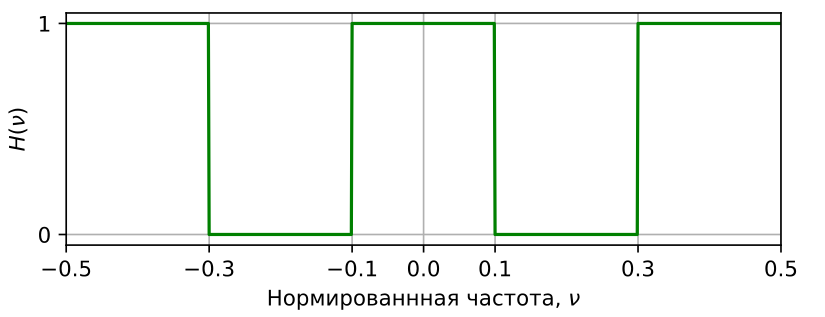
\includegraphics[width=0.6\columnwidth]{pics/fall/7/7-1.png}
		\label{fig:7-1}
		
	\end{figure}
	
\end{itemize}

Заметим, что $\Capit{H}(\nu) = 1 - \Capit{H}_{\ell}^{\nu_1}(\nu) + \Capit{H}_{\ell}^{\nu_2}(\nu)$, где $\Capit{H}_{\ell}^{\nu_c}(\nu)$ -- частотная характеристика идеального фильтра нижних частот с частотой среза $\nu_c$, $\nu_1 = 0.3$ и $\nu_2 = 0.1$. 
В силу линейности ДВПФ справедливо, что $h[k] = \mathbf{1}[k] - h_{\ell}^{\nu_1}[k] + h_{\ell}^{\nu_2}[k]$, где $h_{\ell}^{\nu_c}[k]$ -- импульсная характеристика идеального фильтра нижних частот с частотой среза $\nu_c$. В итоге получим:


\begin{equation*}
	h[k] = \mathbf{1}[k] - h_{\ell}^{\nu_1}[k] + h_{\ell}^{\nu_2}[k] =
	\mathbf{1}[k] - \dfrac{\sin(2 \pi \nu_1 k)}{\pi k} + \dfrac{\sin(2 \pi \nu_2 k)}{\pi k} = 
	\mathbf{1}[k] - \dfrac{2\sin\left(\pi(\nu_1 - \nu_2)k\right)\cos\left(\pi(\nu_1 + \nu_2)k\right)}{\pi k}.
\end{equation*}

$h[k]$ не обращается тождественно в нуль при $k<0$, т.е. не является каузальной. Это означает, что данный фильтр физически не реализуем в системе реального времени. 

\begin{itemize}
	
	\item Идеальный фильтр с нулевой фазовой задержкой, частотная характеристика которого изображена на рисунке.
	\begin{figure}[!h]
		\centering
		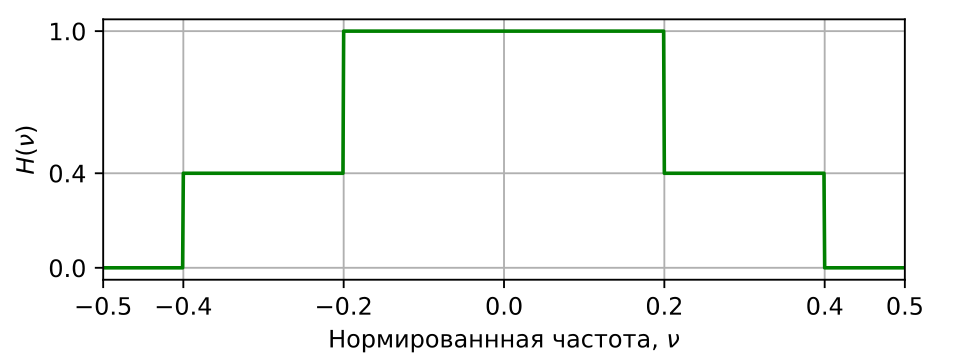
\includegraphics[width=0.6\columnwidth]{pics/fall/7/7-2.png}
		\label{fig:7-2}
	\end{figure}
\end{itemize}

Заметим, что $\Capit{H}(\nu) = 0.4\cdot \Capit{H}_{\ell}^{\nu_1}(\nu) + 0.6 \cdot \Capit{H}_{\ell}^{\nu_2}(\nu)$, где $\nu_1 = 0.4$ и $\nu_2 = 0.2$. 
В силу линейности ДВПФ справедливо, что $h[k] = 0.4 \cdot h_{\ell}^{\nu_1}[k] + 0.6\cdot h_{\ell}^{\nu_2}[k]$. В итоге получим:

\begin{equation*}
	h[k] = 0.4 \cdot h_{\ell}^{\nu_1}[k] + 0.6\cdot h_{\ell}^{\nu_2}[k] = \dfrac{4\sin(2 \pi \nu_1 k) + 6\sin(2 \pi \nu_2 k)}{10\pi k}.
\end{equation*}

$h[k]$ не обращается тождественно в нуль при $k<0$, т.е. не является каузальной. Это означает, что данный фильтр физически не реализуем в системе реального времени. 


\section{}
Определить реакцию на входное воздействие $x[k] = \cos(2\pi \nu_1 k) + \cos(2 \pi \nu_2 k)$, $\nu_1 = 0.1$, $\nu_2 = 0.3$ системы с нулевой фазовой задержкой и амплитудно-частотной характеристикой, изображённой на рисунке (частотная характеристика принимает неотрицательные значения).
\begin{figure}[!h]
	\centering
	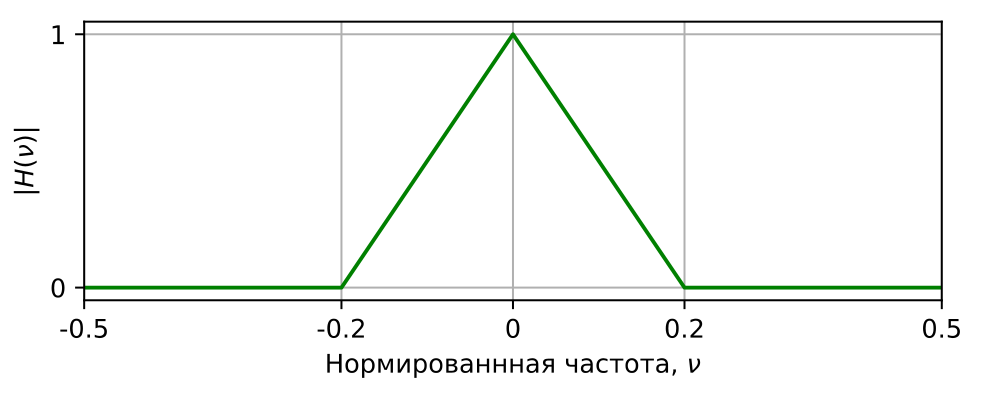
\includegraphics[width=0.6\columnwidth]{pics/fall/7/7-3.png}
	\label{fig:7-3}
\end{figure}

\begin{equation*}
	x[k] \xlongleftrightarrow{DTFT} \Capit{X}(\nu) = \dfrac{1}{2}\sum\limits_{m = \infty}^{+\infty}
	\left[\delta(\nu - \nu_1 + m) + \delta(\nu + \nu_1 + m) + \delta(\nu - \nu_2 + m) + \delta(\nu + \nu_2 + m)\right].
\end{equation*}

\begin{align*}
	\Capit{Y}(\nu) &= \Capit{X}(\nu) \cdot \Capit{H}(\nu) = \dfrac{1}{2}\sum\limits_{m = -\infty}^{+\infty}
	\Capit{X}(\nu) \left[\delta(\nu - \nu_1 + m) + \delta(\nu + \nu_1 + m) + \delta(\nu - \nu_2 + m) + \delta(\nu + \nu_2 + m)\right] = \\
	&= \Big\slash \Capit{X}(\nu_1) = \frac{1}{2},\; \Capit{X}(\nu_2) = 0 \Big\slash = \dfrac{1}{4}\sum\limits_{m = -\infty}^{+\infty}
	\left[\delta(\nu - \nu_1 + m) + \delta(\nu + \nu_1 + m)\right] \xlongleftrightarrow{DTFT} 
	y[k] = \dfrac{1}{2}\cos(2 \pi \nu_1 k).
\end{align*}
